 \documentclass[conference]{IEEEtran}
\IEEEoverridecommandlockouts
% The preceding line is only needed to identify funding in the first footnote. If that is unneeded, please comment it out.
\usepackage{cite}
\usepackage{amsmath,amssymb,amsfonts}
\usepackage{algorithmic}
\usepackage{graphicx}
\usepackage{float} 
\usepackage{subfigure} 
\usepackage{textcomp}
\usepackage{xcolor}
\def\BibTeX{{\rm B\kern-.05em{\sc i\kern-.025em b}\kern-.08em
    T\kern-.1667em\lower.7ex\hbox{E}\kern-.125emX}}
\begin{document}

\title{Software Specification: Tripedia\\
}

\author{\IEEEauthorblockN{Yulin Zhang}
\IEEEauthorblockA{\textit{7th Group} \\
\textit{Software Engineering}\\
Montreal, Canada \\
silveralex2023820@gmail.com}
\and
\IEEEauthorblockN{Yuhang Chen}
\IEEEauthorblockA{\textit{7th Group} \\
\textit{Software Engineering}\\
Montreal, Canada \\
yuhang.chen@mail.concordia.ca}
\and
\IEEEauthorblockN{Jiaxi Yang}
\IEEEauthorblockA{\textit{7th Group} \\
\textit{Software Engineering}\\
Montreal, Canada \\
yjxyang2@outlook.com}
\and
\IEEEauthorblockN{Boyang Wang}
\IEEEauthorblockA{\textit{7th Group} \\
\textit{Software Engineering}\\
Montreal, Canada \\
wangboyang0626@outlook.com}
}

\maketitle


\begin{figure*}[htbp]
\centerline{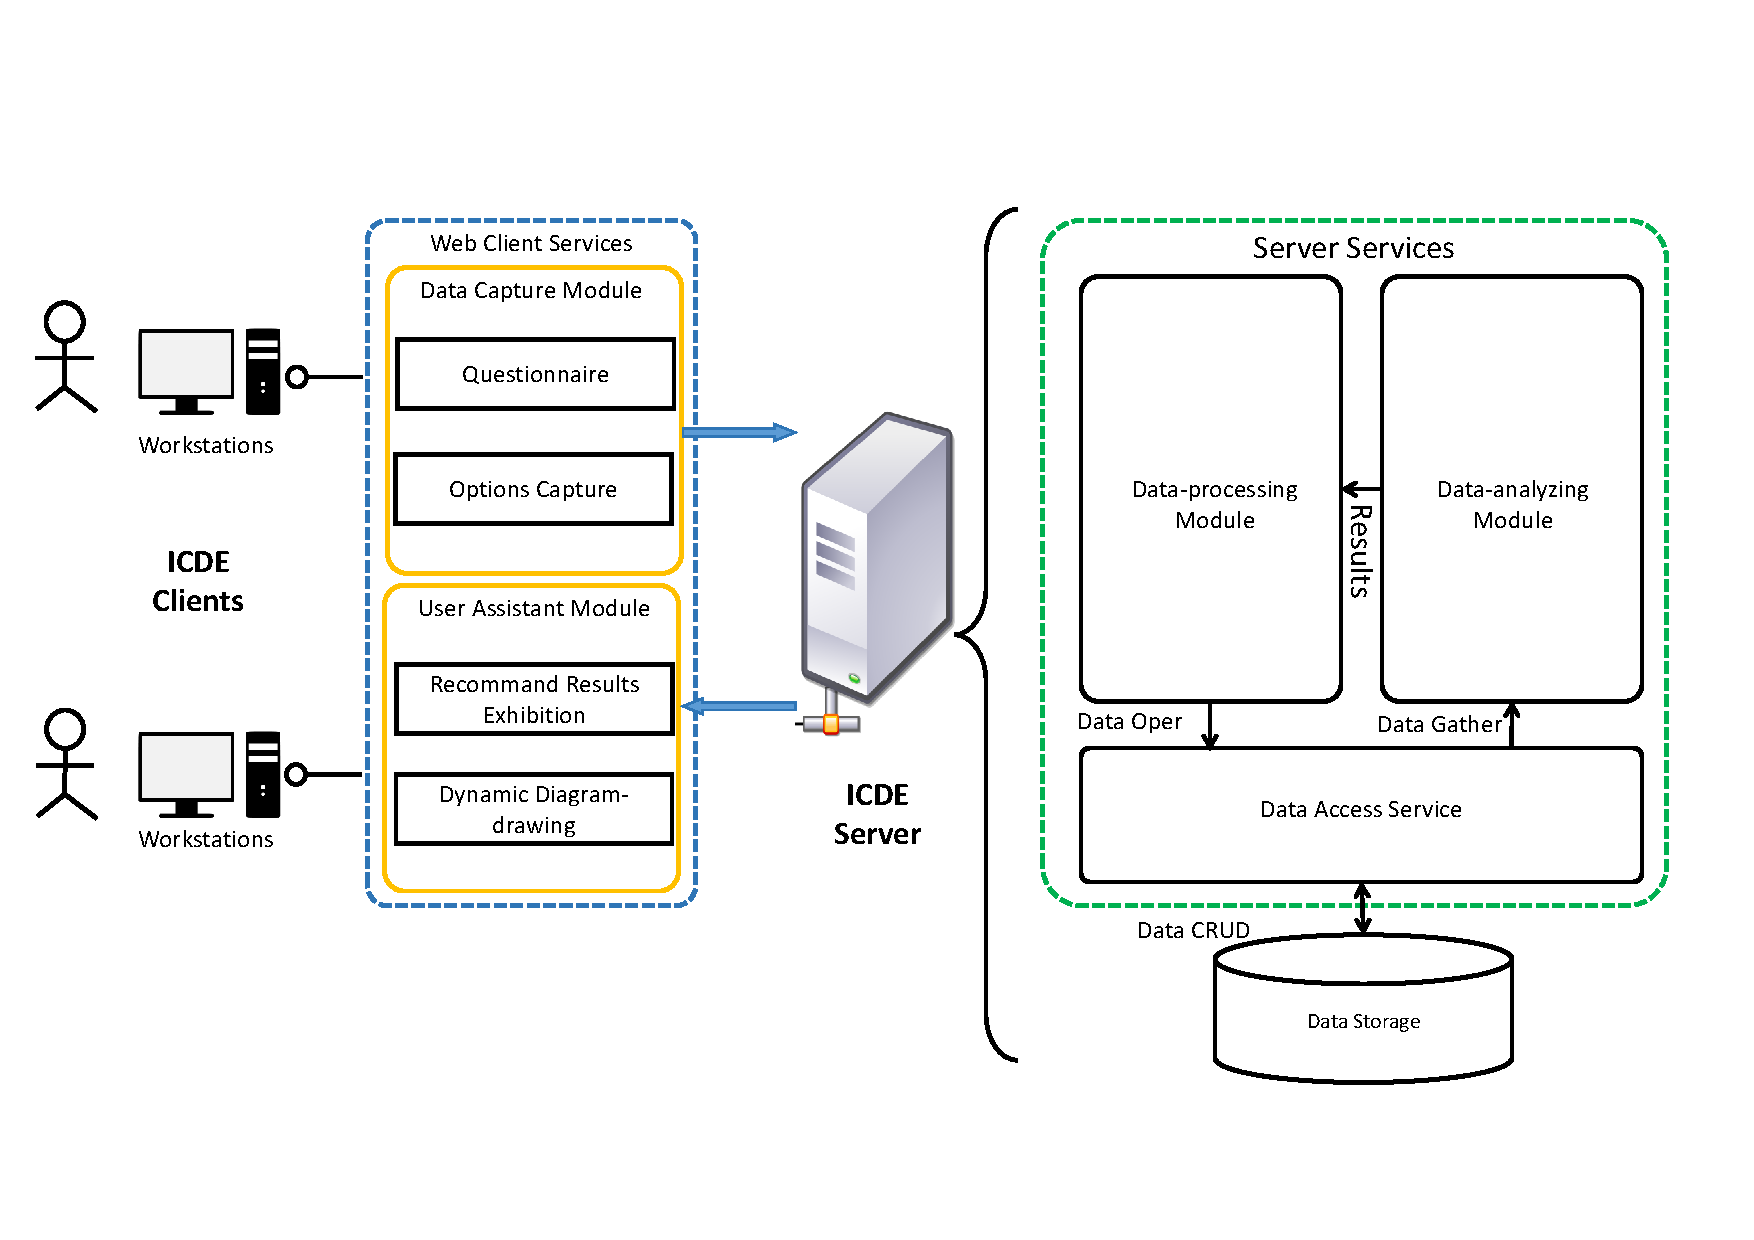
\includegraphics[width=0.9\textwidth]{Architecture.pdf}}
\caption{The architecture graph of Tripedia.}
\label{fig1}
\end{figure*}

\section{Introduction}


\subsection{Problem Statement}

Travel has gradually become an indispensable part of people's lives. According to relevant research, 83\% of Canadians will travel to different cities to experience different customs during their holidays. Travel planning has become a problem that troubles most Canadians. At the same time, many people don’t know which places are more suitable for them. Therefore, travel recommendations and planning have become essential issues affecting people's quality of life.


\subsection{Architecture Design}

As shown in Figure\ref{fig1}, the ICDE system architecture mainly contains two parts: client and server. Based on the limited server hardware equipment, we implement the data analysis logic as a single module in the server, which stands for ICDE 3rd Party Applications. 

In the client part, we implement Tripedia's client logic based on the web. The web client service is mainly divided into two parts: the Data Capture Module and User Assistant Module. The Data Capture Module captures the user's behavior and personal information through questionnaires and behavior captures, and transmits the relevant information to the server. The User Assistant Module is responsible for displaying processed data sent by the server, such as recommendation results and data analysis results, which help users make decisions easily.

On the server side, we will develop three modules to implement the backbone of the ICDE system: Data-processing Module, Data-analyzing Module, and Data Access Service. The Data Access Service, as the median layer for database access, provides a unified database interface (deletion, modification, query, etc) for the Data-processing Module and the Data-analyzing module. The Data-processing Module is responsible for the basic logic of the server, such as registration, login, search, data preprocessing, and other interaction logic with the client. The Data-analyzing Module accesses the data in the database through the Data Access Service to perform data analysis and returns the analysis results to the Data-processing Module.

To sum up, Tripedia's architecture is a standard ICDE system. The Client part includes a Data Capture Service to collect user behavior and information and transmit relevant data to the server. The Data-processing Module in the Servers section is responsible for implementing the interactive logic of the server; the Data Access Service provides a unified data access interface; the Data-analyzing Module serves as the core of the ICDE system to analyze user data and feedback the analysis results to the user through the server to provide User Assistance Service.

\section{Overview}



\subsection{Project Goal}

The goal of the project is to solve the travel planning difficulties faced by users. In response to travel planning issues, this project set out to develop search features to help users. Meanwhile, some users don’t know where is more suitable for travel. This project provides clear charts through the background data analysis function to help users make better decisions. 

\subsection{Key Functionalities}

\textbf{Search} The search feature is responsible for obtaining search results based on the user's search keywords and collected user preferences. This function includes searching for tourist cities, searching for hotels, etc. The search function can provide users with travel route planning.

\textbf{Data Analysis} The website provides a data analysis function if the user doesn't know where is better for vacation. Based on current user preferences and existing data in the system, the website provides data analysis charts of tourist cities suitable for users to help users make better decisions.

\subsection{User Stories}


1. The traveler opens the travel website without logging in, the website will collect his location, so that the website can show local people's favorite place to visit which provides a reference for the user.

2. The traveler registers an account and login to the Tripedia website.

3. The traveler finishes a questionnaire so that the website can recommend appropriate information for users based on the questionnaire content.

4. The traveler has no idea about the where is the best places for him. He finds the data analysis diagram panel for more information to make a decision.

5. The traveler searches for his destination and then the website recommends related information (e.t. hotel, transport function, Landmark Tickets, scenic spot review) so that he can make plans by reference.

6. The traveler checks suitable hotel timings so that he can book an appropriate hotel.

7. The traveler checks suitable flight or train timing so that he can book an appropriate transport function.

8. The traveler selects his favorite hotel and then clicks to jump to the booking screen so that he can make payment.



\subsection{User Cases}


\subsubsection{User Cases: Open Website}

\textbf{ }

\textbf{Use Case}: Open Website.

\textbf{Actors}: Traveler, Server.

\textbf{Summary Description}: Allows any travelers to open Tripedia, and Tripedia shows some basic information about traveling according to the traveler's position.
 
\textbf{Status}: Medium level of details.

\textbf{Pre-condition}: Traveler has to register an account and log in to the Tripedia website to use its service.

\textbf{Post-condition}: The traveler has to have a personal computer and an available network environment.

\textbf{Basic-Path}:

1. The traveler enters the Tripedia website in a browser.

2. The server recommends the travel information entry based on the user's position.

3. The website displays the available travel information sent by the server.

\textbf{Alternate Paths}:

None.

\subsubsection{User Cases: Register and Login}

\textbf{ }

\textbf{Use Case}: Register and Login

\textbf{Actors}: Traveler, Server.

\textbf{Summary Description}: Allows any traveler to register an account and log in to the Tripedia website.
 
\textbf{Status}: Medium level of details.

\textbf{Pre-condition}: The traveler has to open the Tripedia website without login.

\textbf{Post-condition}: Traveler has to complete the questionnaire to use Tripedia's full service.

\textbf{Basic-Path}:

1. The traveler clicks the "register" button on the home page.

2. The website enters the register page

3. The traveler fills in the register information: user name, nationality, gender, and password. 

4. The traveler clicks the "submit" button.

5. The server validates the username is repetitive in the database.

6. The server saves the register information to the database.

7. The website displays the "register successfully" information and enters the login page.

8. The traveler clicks the "login" button on the home page.

9. The traveler fills in the user information, name, and password. 

10. The traveler clicks the "login" button.

11. The server validates the username with the password.

12. The website enters the home page.


\textbf{Alternate Paths}:

5a. The user name is repetitive in the system.

11a. User forgets username/password.

11b. Invalid username/password.

\subsubsection{User Cases: Questionnaire}

\textbf{ }

\textbf{Use Case}: Questionnaire

\textbf{Actors}: Traveller, Server.

\textbf{Summary Description}: Allows any traveler within the login state to have opportunities to complete the questionnaire to get appropriate recommendations.
 
\textbf{Status}: Medium level of details.

\textbf{Pre-condition}: Traveler must be in login state.

\textbf{Post-condition}: Traveler has to user the search function to get more information.

\textbf{Basic-Path}:

1. The website pops up a dialog to ask the user to fill out a questionnaire.

2. The traveler clicks "yes", and the website enters the questionnaire page.

3. The traveler can complete questions about preference.

4. The traveler clicks the "submit" button.

5. The server stores the preference data in the Database.

\textbf{Alternate Paths}:

2a. The user abandons the chance to complete the questionnaire.


\begin{figure}[htbp]
\centerline{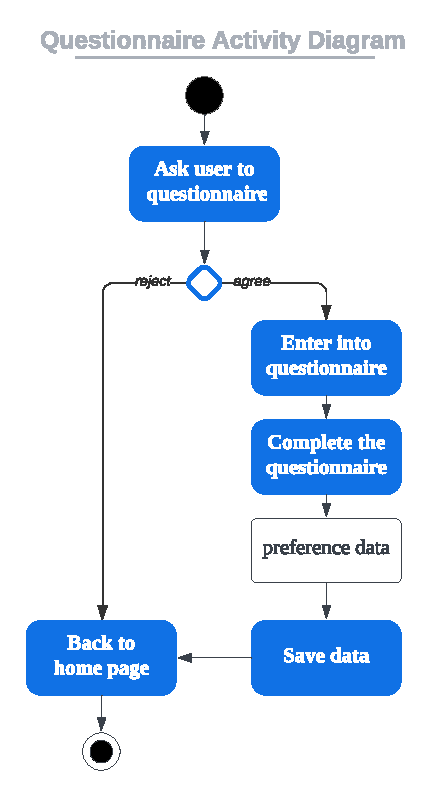
\includegraphics[width=0.3\textwidth]{activity_diagram_question.pdf}}
\caption{The activity diagram of Questionnaire User Case.}
\label{fig2}
\end{figure}


\subsubsection{User Cases: Data Analysis Diagram}

\textbf{ }

\textbf{Use Case}: Data Analysis Diagram

\textbf{Actors}: Traveller, Server, Data Analyzing System.

\textbf{Summary Description}: Allows any traveler within the login state to check the data analysis diagram.
 
\textbf{Status}: Medium level of details.

\textbf{Pre-condition}: Travelers must be in login state and the website is on the home page.

\textbf{Post-condition}: Travelers can search the recommended cities in the search area for more information.

\textbf{Basic-Path}:

1. The traveler clicks the "Analysis Panel" button.

2. The client enters the Data Analysis Page.

3. The data analyzing system analyzes the user's preference data.

4. The server processes the analyzed data.

5. The website displays the diagrams of recommended cities, such as the visitors' number, the visitors' nationalities proportion, etc.

\textbf{Alternate Paths}: None.

\begin{figure}[htbp]
\centerline{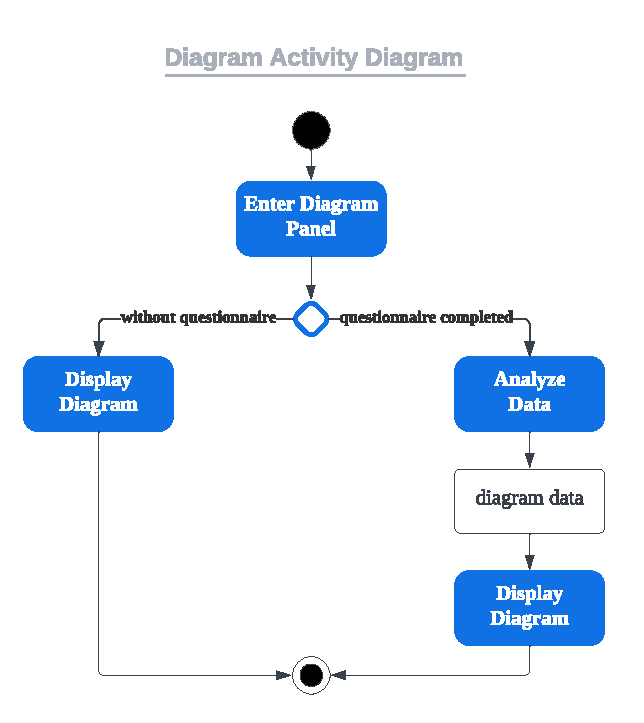
\includegraphics[width=0.5\textwidth]{activity_diagram_diagram.pdf}}
\caption{The activity diagram of Data Analysis Diagram User Case.}
\label{fig3}
\end{figure}


\subsubsection{User Cases: Recommend related information}

\textbf{ }

\textbf{Use Case}: Recommendation

\textbf{Actors}: Traveler, Server, Data Analyzing System.

\textbf{Summary Description}: Allows any traveler to search for his destination, then the website recommends related information.

\textbf{Status}: Medium level of details.

\textbf{Pre-condition}: The traveler has to open the Tripedia website.

\textbf{Post-condition}: The website displays the relevant recommendation information.

\textbf{Basic-Path}:

1. The user enters the website.

2. The user enters the traveling destination in the input box.

3. The user clicks the 'search' button.

4. The data analyzing system analyzes the preference data of the user.

4. The server processed the analyzed data.

5. The website displays the relevant recommendation information in the form of a list.

\textbf{Alternate Paths}:  None

\subsubsection{User Cases: Search hotels}

\textbf{ }

\textbf{Use Case}: Search Hotels

\textbf{Actors}: Traveler, Server.

\textbf{Summary Description}: Allows any traveler to search appropriate hotels.

\textbf{Status}: Medium level of details.

\textbf{Pre-condition}: Travelers must be in login state and the website is on the home page.

\textbf{Post-condition}: The website displays the appropriate hotels list.

\textbf{Basic-Path}:

1. The user enters the website.

2. The user enters the destination in the input box.

3. The user chooses the check-in date and check-out date from the date form.

4. The user clicks the 'search' button.

5. The server collects the target hotels' data.

5. The website displays suitable hotels.

\textbf{Alternate Paths}: None

\subsubsection{User Cases: Search Transportation Tickets}

\textbf{ }

\textbf{Use Case}: Search Transportation Tickets

\textbf{Actors}: Traveler, Server.

\textbf{Summary Description}: Allows any traveler to search for the right mode of transportation

\textbf{Status}: Medium level of details.

\textbf{Pre-condition}: The traveler has to open the Tripedia website.

\textbf{Post-condition}: The user can choose his favorite transportation function.

\textbf{Basic-Path}:

1. The user enters the website.

2. The user enters the destination in the input box.

3. The user chooses departure time and return time from the date-form.

4. The user clicks the 'search' button.

5. The server collects the transportation data. (include flights or trains)

6. The website displays suitable tickets. 


\textbf{Alternate Paths}: None

\subsubsection{User Cases: Check Hotels}

\textbf{ }

\textbf{Use Case}: Check Hotels

\textbf{Actors}: Traveller, Server.

\textbf{Summary Description}: Allows any traveler to check the details of the hotel.

\textbf{Status}: Medium level of details.

\textbf{Pre-condition}: The traveler has to open the Tripedia website.

\textbf{Post-condition}: The user clicks one of the hotels, and the website jumps to a new page of hotel booking details.

\textbf{Basic-Path}:

1. The user enters the website.

2. The user enters the destination in the input box.

3. The user chooses the check-in date and check-out date from the date form.

4. The user clicks the 'search' button.

5. The server collects the hotel's data

6. The website displays suitable hotels.

\textbf{Alternate Paths}: None



\subsection{User Case Diagram}


\begin{figure}[htbp]
\centerline{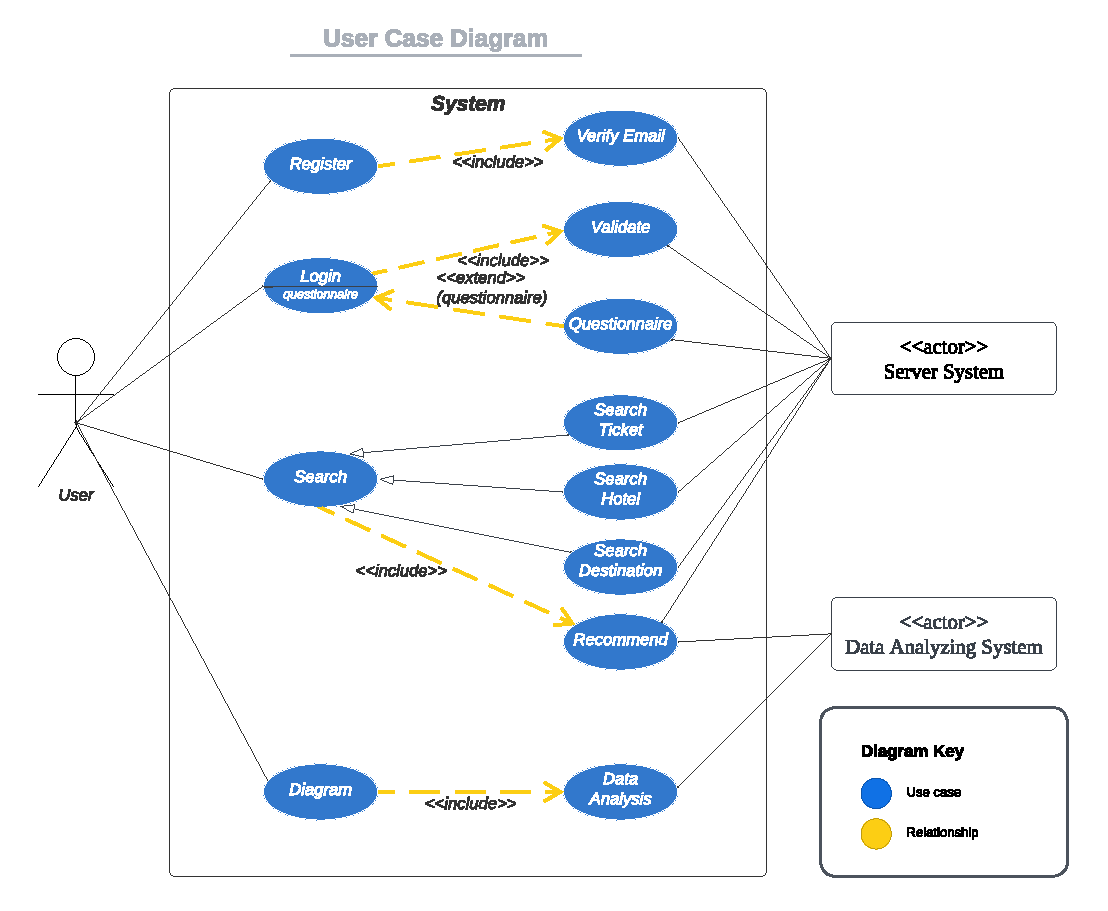
\includegraphics[width=0.5\textwidth]{UserCaseDiagram.pdf}}
\caption{The user case diagram of Tripedia.}
\label{fig2}
\end{figure}



\section{Functional Requirements}

\subsection{ The Requirements Ordering }

We should consider the importance of each requirement and confirm the ordering of requirements.
We divide the requirements into two types: \textbf{mandatory} and \textbf{optional}. A mandatory requirement 
is essential in the system, so these requirements are the first targets to implement for us.
As for optional requirements, these requirements are designed to improve the usability and consummate
the functions in the system. We would like to complete these requirements in the incremental stage.


\subsection{ Login (mandatory)}

As the user case: Register and Login shows, the requirement of Login is an essential functional feature. If users have their accounts, they can log in to the website and get all services. This requirement can be divided into three sub-requirements: 
Enter Username and Password, Validation, and Edit Personal Information.

\subsubsection{ Enter Username and password(mandatory)}

The users can enter their username and password in the input box. The 
user can click on the Show Password button in the password box. When the user 
clicks on this button, the password will be displayed in plaintext in the password 
box so that the user can check if the password is correct before logging in.

\subsubsection{ Validation(mandatory) }

When the user clicks on the login button if the user enters an incorrect 
password or username, the message "Username or password error" will be 
displayed. If the user enters the correct username and password, the system 
will automatically jump to the home page, and the user's login status will be 
displayed on the home page.


\subsection{  Register(mandatory)}

Users can create a new account by entering a username, name, password, email,
and other relevant personal information. This requirement can be divided into 
two sub-requirements: Enter Personal Information, and Verify Email Address.

\subsubsection{ Enter Personal Information(mandatory)}

When the user clicks on the register button on the home page, the page will display several 
input fields to let the user enter his personal information. After finishing the 
input, the user can click the “Register” button to create a new account.

\subsubsection{ Verify Email Address(mandatory) }

After the user inputs their email address, they can click the “Verify the 
email” button, and then the system will send an email to the address. The user
should open the email and click the link in the email to finish the registration. If 
the user doesn't receive the email, they can click the “don’t receive the email” 
button and the system will send the verification email again.

\subsection{ Edit Personal Information(optional) }

\subsubsection{ Change Password(optional) }

When the user wants to change their password, they can enter their 
account page, and click “Change the password” to edit it. The user needs to 
type the old password first to ensure safety. If the user inputs the wrong 
password, a system will display the message “ wrong password. You can’t 
change the password.” If the password is right, the user can type the new 
password and they should input it for the second time to confirm the new
password. After confirming the new password, the user clicks on the “Save”
button to save the change.

\subsubsection{ Update Email Address(optional) }

When the user wants to change their email address, they can enter their 
account page, and click “Change the email address” to edit it. The user can 
input the new email address and click the “Verify the email” button, and then the 
system will send an email to the address. The user should open the email and 
click the link in the email to finish the update. If the user doesn't receive the 
email, they can click the “don’t receive the email” button, and the system will 
send another email.

\subsubsection{ Edit Other Information(optional) }

When the user wants to change other personal information, they can 
enter their account page to edit it. After inputting the new information, click 
the “Save” button to save the edit.

\subsection{ Search(mandatory) }

Users can enter keywords, locations, or other criteria to search for travel 
destinations.
A list of related travel destinations is displayed and the user can click to view 
details.

\subsubsection{ Search Method(mandatory) }

Users should be able to search for the information by using the search 
bar. When users are typing, the system will list the related entries under the 
search bar to help users to search. Moreover, Users should be able to use 
filters and restrictions to narrow down search results. The system should be 
able to save the user's search history so that the user can quickly find the 
required information the next time.

\subsubsection{ Search Result Display(mandatory) }

Search results should be clear and sorted in order of relevance so that 
users can quickly find the information they need. When there are too many 
search results, pagination should be supported. Users can enter the details 
page by displaying the results, which introduces specific information about 
the scenic spot, and the user can enter the official page of the tourist 
destination through the link displayed on the website to learn more.

\subsection{ Data Analysis Diagram(mandatory) }

As the User Cases: Data Analysis Diagram shows, users can check the 
data analysis diagrams calculated by the ICDE system. Meanwhile, the precondition of the Data Analysis Diagram is the Questionnaire, 
so the data analysis diagram requirement combines the processing of the diagram and questionnaire. Furthermore, the Data Analysis
Diagram requirements can be divided into three sub-requirements: Questionnaire, Data Analysis, and Diagram Display.

\subsubsection{ Questionnaire(mandatory) }

When the user first logs in to the website, the website pops up a diagram asking the user to complete a questionnaire to 
get an accurate recommendation. If the user chooses 
to complete the questionnaire, the system will jump to the questionnaire page. The questionnaire page contains several one-choice questions, and
at the end of the page, there is a submit button and a quit button. If the user clicks the "quit" button, the website jumps to the home page.
After completing the questionnaire, the website will send the 
questionnaire information to the data-analyzing module. At the same time, the server program(data-processing module in architecture diagram) 
save the questionnaire information to the database.

\subsubsection{ Data Analysis(mandatory) }

The sub-requirement of Data Analysis is not visible to users, but it is an essential requirement in an ICDE system. While the information on the questionnaire has been sent to
the data-analyzing module, the data-analyzing module will calculate the recommendation weights of cities based on the user's information. We will design a KNN algorithm as the core 
algorithm for data analysis.  


\subsubsection{ Diagram Display(mandatory) }

When the user clicks the "Analysis Panel" button on the home page, the website jumps to the diagram display page.
The website receives the information processed by the data-analyzing module and shows the results by several diagram types. 
The diagrams are initially designed as follows:

\begin{itemize}
\item[*] The most appropriate travel destination: pie chart.

\item[*] The most popular travel destination: bar chart.
\end{itemize}






\section{Nonfunctional Requirements}

\iffalse
\subsection{ Performance }

To cope with high concurrency scenarios, it ensures that users still 
get fast responses during high loads, while maximizing the utilization of the server 
resources. The system should be able to support multi-threaded processing, 
making full use of the server's multi-core resources to improve response speed 
and processing efficiency.
\fi

\subsection{ Usability }

The website's interface should be easy to use, clear, and appropriate for all 
age groups of users. The user interface should be simple and intuitive. Elements 
such as color, fonts, and layout should all contribute to the user experience.
When the user enters incorrect information, there will be a clear error message 
to guide the user on how to correct the error.

\subsection{ Security }

To ensure the security of user passwords, the system performs a hash 
processing to encrypt the passwords instead of storing them in the database in 
plaintext.


\subsection{ Compatibility }


\subsubsection{ Browser compatibility }


The website is compatible with mainstream browsers such as Chrome, 
Firefox, Safari, etc.

\subsubsection{ Operate System compatibility }

Users can access the server page through computer operating systems 
such as Linux, Windows, macOS, and mobile device operating systems such 
as iOS and Android.









\end{document}
